\documentclass[a4paper]{article}
\usepackage{student}
\usepackage{graphicx}

\usepackage{cancel}

% Metadata
\date{\today}

%-------------------------------%
% Other details
% TODO: Fill these
%-------------------------------%
\title{Taller 3}
\setmembername{Cristian Camilo Pérez Puentes,Laura Ximena Rodríguez Quintero,Juan José Ruiz}


%-------------------------------%
% Add / Delete commands and packages
% TODO: Add / Delete here as you need
%-------------------------------%
\usepackage{amsmath,amssymb,bm}
\usepackage[spanish]{babel}

% Custom your usual commands here. Renew these.
\newcommand{\KL}{\mathrm{KL}}
\newcommand{\R}{\mathbb{R}}
\newcommand{\E}{\mathbb{E}}
\newcommand{\T}{\top}
\newcommand{\expdist}[2]{%
        \normalfont{\textsc{Exp}}(#1, #2)%
    }
\newcommand{\expparam}{\bm \lambda}
\newcommand{\Expparam}{\bm \Lambda}
\newcommand{\natparam}{\bm \eta}
\newcommand{\Natparam}{\bm H}
\newcommand{\sufstat}{\bm u}

% Main document
\begin{document}
    % Add header
    \header{}

    % Use `answer` environment to add solutions
    % \begin{answer}[Question 1.1] for example starts an environment formatted
    % for Question 1.1
    \section{La distribución de Maxwell-Boltzmann}
    ¿Cuál es la probabilidad de hallar en un gas ideal que el momentum de una partícula se sale
del promedio? Considere un gas ideal de N partículas esféricas de masa m en un volumen V.\\
    a) Halle el volumen en el espacio de fase $\sum_{\text {esfera }}(E)$ de todos los estados con energía menor o igual a E. (Ayuda: Recuerde que la proyección de estos estados en el espacio de momentos corresponde a una esfera de radio $R=\sqrt{2 m E}$ en $3 \mathrm{~N}$ dimensiones, y que el volumen de una esfera en $n=3 N$ dimensiones es
$$
\pi^{n / 2} \frac{R^n}{\Gamma\left(\frac{n}{2}+1\right)}
$$
    \begin{answer}[literal a]
    Como el espacio de fase $6N$ dimensional dimensional, con $N$ el numero de particulas, se puede considerar como el producto cartesiano del espacio de configuraciones $3N$ dimensional
    y el espacio de momentos $3N$ dimensional, lo cual implica que es valido considerar por separado el volumen espacio de configuraciones y el volumen del espacio de momentos, de fomra 
    tal que el volumen total del espacio de fase es el producto de estos dos volumenes.\\
    El volumen del espacio de configuraciones es el volumen de un $N$-cubo de lado $L^N$, es decir $V^N$. Esto es asi debido a que un gas ocupa todo el espacion que lo contiene y en el espacion 
    de configuraciones por ejemplo para $1$ particula, tendremos que su volumen es $V$ por lo que para $N$ particulas el volumen sera $V^N$.\\
    El volumen del espacio de momentos es el volumen de una $N$-esfera de radio $\sqrt{2mE}$ el cual corresponde a:
    \begin{align*}
        V_{momentos} &= \frac{\pi^{3N/2}}{\Gamma(3N/2 + 1)} (\sqrt{2mE})^{3N} \\
        &= \frac{\pi^{3N/2}}{\Gamma(3N/2 + 1)} (2mE)^{3N/2} \\
    \end{align*}
    Pues los momentos de las particuals estan bajo la restriccion:
    $$\sum_{i=1}^{3N} p_i^2 = \sqrt{2mE} \qquad (1.a.1)$$
    con cada molecual teniendo $3$ grados de libertad.\\
    De esta forma el volumen del espacio de fase para los estado con energia menor igual que $E$ es:
    \begin{align*}
        V_{T}=V_{configuraciones} V_{momentos} \\
        &= V^N \frac{\pi^{3N/2}}{\Gamma(3N/2 + 1)} (2mE)^{3N/2} \\
        &= V^N \frac{\pi^{3N/2}}{\Gamma(3N/2 + 1)} (2m)^{3N/2} E^{3N/2} \\
    \end{align*}
\end{answer}
    b) Derive $\Sigma_{\text {esfera }}(E)$ con respecto a la energía y divida por $h^3$ para encontrar que el número de microestados con energías en el cascarón esférico entre $E$ y E+dE es
$$
\Omega_{\text {cascaron }}(E) d E=\frac{(2 m) \pi^{3 N / 2}}{h^{3 N} \Gamma\left(\frac{3 N}{2}\right)} R^{3 N-2} V^N d E
$$
    \begin{answer}[literal b]
    Como nos interasan los estados del espacio de fase con energia entre $E$ y $E + dE$ y esta restriccion esta dada unicamente por volumen del espacio de los momentos, es necesario 
    derivar el volumen de la $N$-esfera de radio $\sqrt{2mE}$ con respecto al radio que es la energia $E$, para de esta forma obtener los estados que se encuentran en la frontera de esta
    $N$-esfera. Es proceso el similar al realizado para calcular la superficie de una esfera, el cual consiste en derivar su volumen, con respecto al radio. Por lo que:
    \begin{align*}
        \partial V_T &= \frac{dV_T}{dE}\\
        &= V^N \frac{d}{dE}\left[
            \frac{\pi^{3N/2}}{\Gamma(3N/2 + 1)} (2m)^{3N/2} E^{3N/2}
        \right]\\
        &= V^N \frac{\pi^{3N/2}}{\Gamma(3N/2 + 1)} (2m)^{3N/2} \frac{3N}{2} E^{(3N/2) - 1}\\
    \end{align*}
    Como cada grado de libertad tiene una minima energia proporcional a la constante de planck $h$ y como en el espacio de 
    de fase, digamos para una particula el volumen corresponde $(J.s)^3$ entonces $h^{3N}$ representa el volumen de energia minimo que ocuparian las $3N$ particulas en el espacio de fase,
    de esta manera si las particulas fueran distinguibles el numero de estados posibles en el espacio de fase seria:
    \begin{align*}
        \Sigma(E) &= \frac{1}{h^{3N}}\partial V_T dE= \frac{V^N}{h^{3N}} \frac{\pi^{3N/2}}{\Gamma(3N/2 + 1)} (2m)^{3N/2} \frac{3N}{2} E^{(3N/2) - 1}dE\\
    \end{align*}
    Pero dado que las particulas son indistinguibles, entonces es necesario dividir por la cantidad de permutacione, por lo que:
    \begin{align*}
        \Sigma(E) &= \frac{1}{h^{3N}N!}\partial V_T dE= \frac{V^N}{h^{3N}N!} \frac{\pi^{3N/2}}{\Gamma(3N/2 + 1)} (2m)^{3N/2} \frac{3N}{2} E^{(3N/2) - 1}dE\\
    \end{align*}
    donde:
    \begin{align*}
        g(E) = \frac{1}{h^{3N}N!}\partial V_T\\
    \end{align*}
    es la densidad del numero de estados.\\
    Si $R = \sqrt{E}$ entonces numero de estados posibles en el espacio de fase con energia entre $0$ y $E$ es:

    \begin{align*}
        \Omega_{cascaron} &= g(E) \Delta E\\
        &= \frac{1}{h^{3N}N!}\partial V_T \Delta E\\
        &= \frac{V^N}{h^{3N}N!} \frac{\pi^{3N/2}}{\Gamma(3N/2 + 1)} (2m)^{3N/2} \frac{3N}{2} E^{(3N/2) - 1}\Delta E\\
        &= \frac{3N}{2}\frac{V^N}{h^{3N}N!} \frac{(2m\pi)^{3N/2}}{\Gamma(3N/2) \frac{3N}{2}} R^{3N-2}  \Delta E\\
        &= \frac{V^N}{h^{3N}N!} \frac{(2m\pi)^{3N/2}}{\Gamma(3N/2)} R^{3N-2}  \Delta E\\
    \end{align*}
\end{answer}    
    Ahora pensemos que una componente de momentum está fija, con valor $p_1$. Los estados compatibles con esta condición forman un anillo, que también es un cascarón esférico, pero en $3 \mathrm{~N}-1$ dimensiones, y de radio $R^{\prime}=\sqrt{2 m E-p_1^2}$.
\begin{figure}[h]
    \centering
    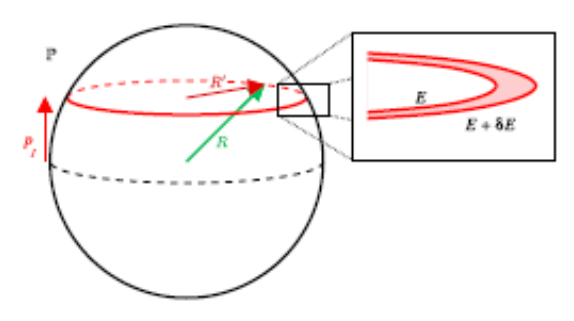
\includegraphics[width=0.5\textwidth]{punto1/cascaron.png}
    \caption{Cascaron esferico en 3 dimensiones}
    \label{fig:my_label}
\end{figure}


    c) $\mathrm{Si}$ asumimos que el anillo tiene un espesor $d p_1$ (no mostrado en la gráfica), derive que el número de microestados en el anillo es
$$
\Omega_{\text {anillo }}=\frac{(2 m) \pi^{(3 N-1) / 2}}{\Gamma\left(\frac{3 N-1}{2}\right)} \frac{R^{\prime 3 N-3} V^N}{h^{3 N}(N-1) !} \Delta E \Delta p_1 .
$$
    Si fijamos $p_1$, es decir que $p_1$ es constante, entonces de la ecuación $(1.a.1)$ tenemos que
\begin{answer}
    \begin{align*}
        \sum_{i=2}^{3N} = 2mE - p_1^2 = \sqrt{2mE - p_1^2}  \qquad (1.c.1)
    \end{align*}
    Lo que define una $3N - 1$ esfera de radio $\sqrt{2mE - p_1^2}$ en el espacio de momentos de $3N - 1$ dimensiones.\\
    El volumen en espacio en espacio de las configuraciones continua siendo $V^N$ pues que el momento $p_1$ sea fijo no implica 
    que la posicion $q_1$ sea fija.\\
    De lo anterior tenemos que el volumen del espacio de fase es(dado que el hamiltoniano es separable):
    \begin{align*}
        V_{T} &= V^N \frac{\pi^{(3N-1)/2}}{\Gamma((3N-1)/2 + 1)} (2mE - p_1^2)^{(3N-1)/2} \\
        &= V^N \frac{\pi^{(3N-1)/2}}{\Gamma((3N-1)/2 + 1)} (2m)^{(3N-1)/2} \left(E - \frac{p_1^2}{2m}\right)^{(3N-1)/2} \\
    \end{align*}
    Y de forma análoga al literal a) el numero de estados posibles con el energia menor o igual que $E - \frac{p_1^2}{2m}$ es:
    \begin{align*}
        g(E)dp &= \frac{1}{h^{3N}(N-1)!} \partial V_T \Delta E ~dp\\
        &= \frac{1}{h^{3N}(N-1)!} V^N \frac{\pi^{(3N-1)/2}}{\Gamma\left(\frac{(3N-1)}2\right)} (2m)^{(3N-1)/2} \left(E - \frac{p_1^2}{2m}\right)^{(3N-1)/2 - 1} \Delta E ~dp\\
    \end{align*}
    Y si $R' = \sqrt{E - \frac{p_1^2}{2m}}$ entonces:
    \begin{align*}
        \Omega_{anillo} &= \frac{V^NR'^{3N-3}}{h^{3N}(N-1)!}  \frac{ (2m\pi)^{(3N-1)/2}}{\Gamma\left(\frac{(3N-1)}2\right)} \Delta E ~\Delta p\\
    \end{align*}
\end{answer}


    d) Demuestre que la probabilidad de hallar el momentum $p_1$ entre $p_1$ y $p_1+d p_1$ es proporcional
$$
P\left(p_1\right) \Delta p_1=\frac{\Omega_{\text {anillo }}}{\Omega_{\text {cascaron }}} \propto \frac{R^{3 N-3}}{R^{3 N-2}}=\frac{1}{R}\left[1-\frac{p_1^2}{2 m E}\right]^{\frac{3 N-3}{2}} \approx \frac{1}{R}[1-\epsilon]^{\frac{3 N}{2}} \quad, \text { con } \quad \epsilon=\frac{p_1^2}{2 m E} .
$$
Como el término entre corchetes cuadrados está elevado a un exponente enorme, la probabilidad será diferente de cero solamente si este término es similar a 1 , es decir, si $p_1 \sim 0$.
    \begin{answer}
    De los lierarles anteriores tenemos que la probabilidad de hallar una partícula con momentum $p_1$ entre $p_1$ y $p_1+dp_1$ es decir $\Delta p_1= dp_1$, es tal que:
    \begin{align*}
        P(p_1)dp &= \frac{\Omega_{anillo}}{\Omega_{cascaron}} \\
        &= \frac{
            \frac{\cancel{V^N}R'^{3N-3}}{\cancel{h^{3N}}(N-1)!}  \frac{ \cancel{(2m\pi)^{(3N-1)/2}}}{\Gamma\left(\frac{3N}2-\frac{1}2\right)}\cancel{\Delta E} ~dp
        }{
            \frac{\cancel{V^N}}{\cancel{h^{3N}}N!} \frac{(2m\pi)^{\cancel{3N/2}}}{\Gamma(3N/2)} R^{3N-2}  \cancel{\Delta E}
        }\\\\
        &=  \frac{
            \frac{R'^{3N-3}}{\cancel{(N-1)!}}  \frac{1}{\Gamma\left(\frac{(3N-1)}2\right)} ~dp
        }{
            \frac{(2m\pi)^{1/2}R^{3N-2}}{\Gamma\left(\frac{3N}2\right)N\cancel{(N-1)!}} 
        }\\\\
        &= \frac{R'^{3N-3}\Gamma\left(\frac{3N}2\right)N}{\Gamma\left(\frac{3N}2-\frac{1}2\right)(2m\pi)^{1/2}R^{3N-2} }dp
    \end{align*}
    De lo cual concluimos que:
    \begin{align*}
        P(p_1)  \propto \frac{R'^{3N-3}}{R^{3N-2}} &= \frac{\left(E-\frac{p_1^2}{2m}\right)^{\frac {3N}2 - \frac 32}}{{E}^{\frac{3N}{2} - 1}}\\
        &= \frac{E^{\frac {3N}2 -\frac 32}}{E^{\frac {3N}2 -1}}\left(1-\frac{p_1^2}{2mE}\right)^{\frac {3N}2 - \frac 32}\\
        &= \frac{E^{\frac {3N}2} E^{-\frac 12} E^{-1}}{E^{\frac {3N}2} E^{-1}}\left(1-\frac{p_1^2}{2mE}\right)^{\frac {3N}2 - \frac 32}\\
        &= \frac{1}{E^{\frac 12}}\left(
            1-\frac{p_1^2}{2mE}
        \right)^{\frac {3N}2 - \frac 32}\\
        &= \frac{1}{R}\left(
            1-\frac{p_1^2}{2mE}
        \right)^{\frac {3N - 3}2} = \frac{1}{R}\left(
            1-\frac{p_1^2}{2mE}
            \right)^{\frac {3N}2 } \left(
            1-\frac{p_1^2}{2mE}
        \right)^{-\frac 32}\\
        &= \frac{1}{R}\left(
            1-\epsilon
            \right)^{\frac {3N}2 } \left(
            1-\epsilon
        \right)^{-\frac 32} = \frac{1}{R}\left(
            1-\epsilon
            \right)^{\frac {3N}2} \frac{1}{\left(
            1-\epsilon
            \right)} \frac{1}{\sqrt{
            1-\epsilon
            }}
    \end{align*}
    Veamos que la en general la energia de ensamble completo es mucho mayor que la energia de una sola molecula de gas, es decir $E \gg \frac{p_1^2}{2m}$, por tanto:
    \begin{align*}
        \frac{1}{(1-\epsilon)} \approx 1 \qquad \text{y} \qquad \frac{1}{\sqrt{1-\epsilon}} \approx 1 \quad \Rightarrow\quad \frac{1}{(1-\epsilon)} \frac{1}{\sqrt{1-\epsilon}} \approx 1
    \end{align*}
    Por lo tanto:
    \begin{align*}
        P(p_1)  &\propto \frac{R^{3N-3}}{R^{3N-2}} \\
        &= \frac{1}{R}\left(
            1-\epsilon
            \right)^{\frac {3N}2 } \frac{1}{\left(
            1-\epsilon
            \right)} \frac{1}{\sqrt{
            1-\epsilon
            }}\\
        &\approx \frac{1}{R}\left(
            1-\epsilon
            \right)^{\frac {3N}2 } 
    \end{align*}
    Por lo que la probabilidad de hallar una partícula con momentum $p_1$ entre $p_1$ y $p_1+dp_1$ es apreciable solo cuando $p_1 \sim 0$.
    Esto significa es muy como probable que una particual tenga la mayor parte de la energia del sistema.
\end{answer}



    e)Usando la aproximación $1-p_1^2 / 2 m E=1-\epsilon \simeq \exp (-\epsilon)$, muestre que, una vez normalizada, la densidad de probabilidad con la que se miden los valores de $p_1$ distribuye aproximadamente como una gaussiana,
    \section{ ¿Qué tan probable es encontrar más moléculas de un gas a 
    un lado que al otro de un salón?}
    Imagine un gas ideal de $n$ moléculas idénticas que se encuentra en una caja de $N$ celdas que podemos dividir mentalmente en dos zonas: una zona izquierda (I) de $I$ celdas, y otra derecha (D) de $D$ celdas. Asumamos que cada celda puede tener a lo más una molécula. Si todas las formas de repartir las $n$ moléculas en las $N$ celdas son igualmente probables, ¿por qué es casi imposible ver que todas las moléculas se coloquen en una de las dos zonas, dejando a la otra vacía? Vamos a estudiar el problema de dos maneras: analítica y computacional.
Para la parte analítica,


    a) Estime la probabilidad $P_l(k)$ de encontrar $k$ moléculas a la izquierda contando todas las maneras posibles de colocar $k$ moléculas en las cajas de la zona I (y, por lo tanto, $l=n-k$ moléculas en la zona $\mathrm{D}$ ) y dividiéndola por el número de maneras posibles de colocar las n moléculas en todas las $N=\mathrm{I}+\mathrm{D}$ cajas. Compruebe que la razón resulta ser,
$$
P_I(k)=\frac{\Omega_I(k) \Omega_D(l)}{\Omega_N(n)},
$$
con
$$
\Omega_l(k)=\left(\begin{array}{l}
I \\
k
\end{array}\right), \quad \Omega_l(k)=\left(\begin{array}{l}
D \\
l
\end{array}\right), \Omega_N(n)=\left(\begin{array}{l}
N \\
n
\end{array}\right)
$$
    \begin{answer}
    Dado un gas ideal de $n$ moléculas idénticas en una caja de $N$ celdas, donde cada celda puede tener a lo más una molécula 
    el conjunto de todos los estados posibles $\Omega_N(n) := \{\text{toda las formas en la que podemos elegir N celdas para colocar n moléculas}\}$,
    si enumeramos las $N$ celdas de $1,\dots,N$ como las moleculas son indistinguibles  entonces no importa que caja almacena que molécula y ningua puede ser seleccionada mas de una vez, entonces 
    $\Omega_N(n) := \{T: T \subset \{1,2,\dots,N\}, |T| = n\}$, por lo tanto 
    \begin{align*}
        \Omega_N(n) := | \Omega_N(n) | = {N \choose n}
    \end{align*}
    y la cantidad estados favorables que consisten de todas las formas en las que podemos elegir $I$ celdas para colocar $k$ moléculas en la zona derecha y por lo tanto $D$ celdas para colocar $l$ es 
    de forma analoga a los casos totales 
    \begin{align*}
        \Omega_D(k) := \Omega_I(l) := |\Omega_I(k)||\Omega_D(l)| = {I \choose k}{D \choose l}
    \end{align*} 
    por lo tanto la probabilidad de encontrar $k$ moleculas en la zona izquierda es:
    \begin{align*}
        P_I(k) &= \frac{\Omega_I(k) \Omega_D(l)}{\Omega_N(n)} = \frac{{I \choose k}{D \choose l}}{{N \choose n}}\\
        &= \frac{{I \choose k}{N-I \choose n-k}}{{N \choose n}}\\
    \end{align*}
    Lo cual corresponde efectivamente a una distribución hipergeometrica de una poblacion de $N$ elementos, donde $I$ son los elementos de la poblacion que son exitos de una muestra de $n$ elementos sin reemplazo. 
\end{answer}

    b) ¿Bajo qué condiciones se maximiza la probabilidad $P_I(k)$ ? Como el denominador $\Omega_N(n)$ es constante y el logaritmo es una función monótona, el máximo se obtiene cuando la entropía total $S(k)=S_I(k)+S_D(l)$ es máxima, $\operatorname{con} S_I(k)=\ln \Omega_I(k)$ y $S_D(l)=\ln \Omega_D(l)$. Derive la entropía total respecto a $k$, iguálela a cero y compruebe que,
$$
\frac{\partial S_I}{\partial k}=\frac{\partial S_D}{\partial l},
$$
que es para nuestro caso la versión de que la entropía se maximiza cuando las "temperaturas" $T_I=\frac{\partial S_I}{\partial k}$ y $T_D=\frac{\partial S_D}{\partial k}$ son iguales.
    \begin{answer}
    Si vemos un ensamble estadistico como $P\subseteq \Omega \times [0,1]$, es decir,
    \begin{align*}
        P: &\Omega \mapsto [0,1]\\
        &\omega \mapsto P(\omega) \in [0,1]
    \end{align*}
    tal que $P := \{(\omega,\rho): \omega \in \Omega \quad \text{y} \quad \rho \in [0,1]\}$ si $\Omega$ es finito y sea $\{p_i\}_{i=1}^n$ un familia de subconjunto de $P$ tal que $p_i \cap p_ j = \emptyset$ para $i\neq j$ y $\bigcup_{i=1}^n p_i = P$ entonces la entropia 
    del ensamble la cual se define como:
    \begin{align*}
        S(P) &= -\sum_{(\omega,\rho) \in P} \rho \log \rho = -\sum_{i = 1}^{|\Omega|} P(\omega_i) \log P(\omega_i)\\
        &= -\sum_{i = 1}^{|\Omega|} \rho_i \log \rho_i
    \end{align*} 
    \begin{enumerate}
        \item $S(P) = S\left(\bigcup_{i=1}^n p_i\right) = \sum_{i=1}^n S(p_i)$
        \item para $i\neq j$ $S(p_i \cup p_j) = S(p_i) + S(p_j)$
    \end{enumerate}
    Para un gas ideal de $n$ moleculas en un volumen $V$ particionado en $N$ celda $V_i$ con $i = 1,2,\dots,N$ y $V = \sum_{i=1}^N V_i$ entonces el cojunto de casos totales es 
    \begin{align*}
        \Omega = \{b_0b_1\dots b_N: b_i \in \{0,1\}\} = \{k: k = b_i 2^i \quad \text{con} \quad b_i \in \{0,1\}\}
    \end{align*}
    con:
    $$
     b_i = \begin{cases}
        1 & \text{si la molecula esta en el celda } V_i\\
        0 & \text{en otro caso}
    \end{cases}
    $$
    Si dividimos le cadena de bits en los primeros $I$ bits con $k$ unos y los ultimos $D = N - I$ bits con $l= n-k$ entoces el numero de formas en las que puedo colocar los $k$ unos en los primeros $I$ bits es:
    \begin{align*}
        |\Omega_I(K)|= \binom{I}{k} = \frac{I!}{k!(I-k)!}
    \end{align*}
    donde:
    \begin{align*}
        \Omega_I(K) &= \{b_0b_1 \dots b_Ic_{I+1}c_{I+2}\dots c_N: b_i \in \{0,1\} \quad \text{y} \quad c_i \in \{0,1\} \text{ fijos}\}\\
        \Omega_I(K) &= \{d_0d_1\dots d_Ib_{I+1}b_{I+2}\dots b_N: b_i \in \{0,1\} \quad \text{y} \quad d_i \in \{0,1\} \text{ fijos}\}\\
    \end{align*}
    entonces el ensamble microcanonico es para $\Omega_I(K)$:
    \begin{align*}
        P_I := \left\{ \left(\omega, \rho \right): \omega \in \Omega_I(K)  \quad \text{y} \quad = \frac{1}{|\Omega_I(K)|}\right\}
    \end{align*}
    De la forma analoga definimos el ensamble microcanonico para $\Omega_D(L)$:
    \begin{align*}
        P_D := \left\{ \left(\omega, \rho \right): \omega \in \Omega_D(L)  \quad \text{y} \quad = \frac{1}{|\Omega_D(L)|}\right\} - \{d_0d_1\dots d_Ic_{I+1}c_{I+2}\dots c_N\}
    \end{align*}
    Veamos que $P_I \cap P_D = \emptyset$ y $P_I \cup P_D = P$ entonces
    \begin{align*}
        S(P) &= S(P_I \cup P_D) = S(P_I) + S(P_D)\\
        &= S(P_I) + S(P_D)\\
        &= \log |\Omega_I(K)| + \log |\Omega_D(L)|\\
        &= \log \binom{I}{k} + \log \binom{D}{l}\\
        &= \log \frac{I!}{k!(I-k)!} + \log \frac{D!}{l!(D-l)!}\\
        &= \log \frac{I!D!}{k!(I-k)!l!(D-l)!}\\
        &= \log \frac{N!}{k!l!(N-k)!(N-l)!}\\
        &= \log \binom{N}{k}
    \end{align*}a
\end{answer}
    c) Compruebe que el valor de $k$ que maximiza la probabilidad $P_I(k)$ se cumple
$$
\frac{k}{I}=\frac{l}{D}=\frac{n}{N} \text {, con lo cual } k_{\max }=n \frac{I}{N} \text {. }
$$
    d) Ahora calculemos la probabilidad de que haya $k=k_{\max }+\varepsilon$ moléculas en la zona izquierda.

    \begin{answer}[punto ]
        Dado que $$P_I(k) = \frac{\Omega_I(k) \Omega_D(n-k)}{\Omega_I(n)}$$
        entonces:
        \begin{align*}
            P_I(k + \epsilon) &= \frac{\Omega_I(k) \Omega_D(n-k)}{\Omega_I(n)} \\
            &= \frac{{I \choose k} {D \choose n - k}}{{N \choose n}} \\
            &= \frac{\frac{I!}{(k)!(I - k)!} \frac{D!}{(n - k)!(D - n + k)!}}{\frac {N!}{n!(N - n)!}} \\
            &= \frac{\frac{I!}{(k)!(I - k)!} \frac{(N-I)!}{(n - k)!(D - n + k)!}}{\frac {N!}{n!(N - n)!}} \\
            &= \frac{I!(N-I)!n!(N-n)!}{(k)!(I - k)!(n - k)!(D - n + k)!N!} \\
            &= \frac{n!(N-n)!}{(k)!(I - k)!(n - k)!((N-I) - n + k)!}\frac{1}{{N \choose I}} \\
            &= \frac{(N-n)!}{(I - k)!((N-I) - n + k)!}\frac{{n \choose k}}{{N \choose I}} \\
            &= \frac{(N-n)!}{(I - k)!((N-n) - (I - k))!}\frac{{n \choose k}}{{N \choose I}} \\
            &= {N-n \choose I - k}\frac{{n \choose k}}{{N \choose I}} \\
        \end{align*}
        Aplicando la aproximacion de logaritmo natural a:
        $$
         \frac{I!(N-I)!n!(N-n)!}{(k + \epsilon)!(I - (k+\epsilon))!(n - k-\epsilon)!((N-I) - n + k+\epsilon)!N!} \\
        $$
        tenemos que:
        \begin{align*}
            &\ln \left[
            \frac{I!(N-I)!n!(N-n)!}{(k + \epsilon)!(I - (k+\epsilon))!(n - k-\epsilon)!((N-I) - n + k+\epsilon)!N!}
            \right] \\
            &= \ln \left[I! (N-I)! n! (N-n)! \right] - \ln \left[(k + \epsilon)! (I - (k+\epsilon))! (n - k-\epsilon)! ((N-I) - n + k+\epsilon)! N! \right] \\
            &= \ln \left(I!\right) + \ln \left((N-I)!\right) + \ln \left(n!\right) + \ln \left((N-n)!\right) \\
            &- \ln \left((k + \epsilon)!\right) - \ln \left((I - (k+\epsilon))!\right) - \ln \left((n - k-\epsilon)!\right) - \ln \left(((N-I) - n + k+\epsilon)!\right) - \ln \left(N!\right)  \\
        \end{align*}
        Y a esto ultimo aplicando la aproximacion de Stirling:
        \begin{align*}
            &\ln \left[
            \frac{I!(N-I)!n!(N-n)!}{(k + \epsilon)!(I - (k+\epsilon))!(n - k-\epsilon)!((N-I) - n + k+\epsilon)!N!}
            \right] \\
            &= I \ln \left(I\right) - \cancel I + ( N-I) \ln \left(N-I\right) - (\cancel N-\cancel I) + n \ln \left(n\right) - \cancel n + (N-n) \ln \left(N-n\right) - (N-\cancel n) \\
            &- (k + \epsilon) \ln \left(k + \epsilon\right) + (k + \epsilon) - (I - (k+\epsilon)) \ln \left(I - (k+\epsilon)\right) + (I - (k+\epsilon)) \\
            &- (n - k-\epsilon) \ln \left(n - k-\epsilon\right) + (n - k-\epsilon) - ((N-I) - n + k+\epsilon) \ln \left((N-I) - n + k+\epsilon\right) \\
            &+ ((N-I) - n + k+\epsilon) - N \ln \left(N\right) +\cancel N \\
            &= I \ln \left(I\right)  + ( N-I) \ln \left(N-I\right) + n \ln \left(n\right)  + (N-n) \ln \left(N-n\right) - \cancel N \\
            &- (k + \epsilon) \ln \left(k + \epsilon\right) + \cancel{(k + \epsilon)} - (I - (k+\epsilon)) \ln \left(I - (k+\epsilon)\right) + (I - \cancel{(k+\epsilon)}) \\
            &- (n - k-\epsilon) \ln \left(n - k-\epsilon\right) + \cancel{(n - k-\epsilon)} - ((N-I) - n + k+\epsilon) \ln \left((N-I) - (n - k-\epsilon)\right) \\
            &+ ((\cancel N-I) -\cancel{(n - k-\epsilon)}) - N \ln \left(N\right)  \\
            &= I \ln \left(I\right)  + ( N-I) \ln \left(N-I\right) + n \ln \left(n\right)  + (N-n) \ln \left(N-n\right)\\
            &- (k + \epsilon) \ln \left(k + \epsilon\right)  - (I - (k+\epsilon)) \ln \left(I - (k+\epsilon)\right)  \\
            &- (n - k-\epsilon) \ln \left(n - k-\epsilon\right) - ((N-I) - n + k+\epsilon) \ln \left((N-I) - (n - k-\epsilon)\right) \\
            & - N \ln \left(N\right) \\
        \end{align*}
        \begin{align*}
            &= I \ln \left(I\right)  + N\ln \left(N-I\right)-I\ln \left(N-I\right) + n \ln \left(n\right)  + N\ln \left(N-n\right)-n\ln \left(N-n\right)\\
            &- k \ln \left(k + \epsilon\right) - \epsilon \ln \left(k + \epsilon\right)  - I \ln \left(I - (k+\epsilon)\right) + k\ln \left(I - (k+\epsilon)\right)  + \epsilon \ln \left(I - (k+\epsilon)\right)  \\
            &- n \ln \left(n - k-\epsilon\right) + k \ln \left(n - k-\epsilon\right) + \epsilon \ln \left(n - k-\epsilon\right) \\
            &- N \ln \left((N-I)\right) -I \ln \left((N-I) - (n - k-\epsilon)\right) - n \ln \left((N-I) - (n - k-\epsilon)\right) \\
            &+ k \ln \left((N-I) - (n - k-\epsilon)\right) + \epsilon \ln \left((N-I) - (n - k-\epsilon)\right) \\
            & - N \ln \left(N\right) \\
            &= I\left[
                \ln \left(I\right)  - \ln \left(N-I\right) - \ln \left(I - (k+\epsilon)\right) + \ln \left((N-I) - (n - k-\epsilon)\right)
            \right]\\
            &+ N\left[
                \ln \left(N-I\right) - \ln \left(N\right)
            \right]\\
            &+ n\left[
                \ln \left(n\right)  - \ln \left(N-n\right) - \ln \left(n - k-\epsilon\right) + \ln \left((N-I) - (n - k-\epsilon)\right)
            \right]\\
        \end{align*}
        entonces
        \begin{align*}
            &\frac{I!(N-I)!n!(N-n)!}{(k + \epsilon)!(I - (k+\epsilon))!(n - k-\epsilon)!((N-I) - n + k+\epsilon)!N!}\\ 
            &=\frac{\sqrt{2\pi I}(\frac{I}{e})^I\sqrt{2\pi (N-I)}(\frac{N-I}{e})^{N-I}\sqrt{2\pi n}(\frac{n}{e})^n\sqrt{2\pi (N-n)}(\frac{N-n}{e})^{N-n}}{\sqrt{2\pi (k + \epsilon)}(\frac{k + \epsilon}{e})^{k + \epsilon}\sqrt{2\pi (I - (k+\epsilon))}(\frac{I - (k+\epsilon)}{e})^{I - (k+\epsilon)}} \\
            &\frac{1}{\sqrt{2\pi (n - k-\epsilon)}(\frac{n - k-\epsilon}{e})^{n - k-\epsilon}\sqrt{2\pi ((N-I) - n + k+\epsilon)}(\frac{(N-I) - n + k+\epsilon}{e})^{(N-I) - n + k+\epsilon}\sqrt{2\pi N}(\frac{N}{e})^N}
        \end{align*}     
    \end{answer}
    $$
    P(x, p)=\frac{2 \pi}{\beta \omega} e^{-\beta\left[\frac{p^2}{2 m}+\frac{1}{2} k x^2\right]},\qquad  \operatorname{con} \beta=\frac{1}{k_B T} \qquad \mathrm{y} \qquad \omega=\sqrt{\frac{k}{m}}
    $$
    Deduzca que la distribución de probabilidad marginal teórica $P(x)$, que se construye integrando la probabilidad de Boltzmann $P(x, p)$ sobre $p$,
    $$
    P(x)=\frac{2 \pi k_B T}{\omega} \int_{-\infty}^{\infty} e^{-\beta\left[\frac{p^2}{2 m}+\frac{1}{2} k x^2\right]} d p,
    $$
    es una gaussiana centrada en cero con desviación estándar $\sigma_x=\sqrt{k_B T / k}$. De manera similar, demuestre que la distribución de probabilidad marginal teórica $P(p)$, que se construye integrando la probabilidad de Boltzmann $P(x, p)$ sobre $\mathrm{x}$,
    $$
    P(p)=\frac{2 \pi k_B T}{\omega} \int_{-\infty}^{\infty} e^{-\beta\left[\frac{p^2}{2 m}+\frac{1}{2} k x^2\right]} d x,
    $$
    resulta ser una gaussiana con media cero y desviación estándar $\sigma_p=\sqrt{m k_B T}$.

    \begin{answer}
        \begin{align*}
            P(x) &= \frac{2 \pi k_B T}{\omega} \int_{-\infty}^{\infty} e^{-\beta\left[\frac{p^2}{2 m}+\frac{1}{2} k x^2\right]} d p \\
            &= \frac{2 \pi k_B T}{\omega} \int_{-\infty}^{\infty} e^{-\beta\left[\frac{p^2}{2 m}+\frac{1}{2} k x^2\right]} d p \\
            &= \frac{2 \pi k_B T}{\omega} \int_{-\infty}^{\infty} e^{-\beta\left[\frac{p^2}{2 m}\right]} e^{-\beta\left[\frac{1}{2} k x^2\right]} d p \\
            &= \frac{2 \pi k_B T}{\omega} e^{-\beta\left[\frac{1}{2} k x^2\right]} \int_{-\infty}^{\infty} e^{-\beta\left[\frac{p^2}{2 m}\right]} d p \\
        \end{align*}
        Si $z^2 = \beta \frac{p^2}{2m}$ entonces $z= p\sqrt{\beta \frac{1}{2m}}$ y $d z = \sqrt{\beta \frac{1}{2m}} d p$ por lo que:

        \begin{align*}
            P(x) &= \frac{2 \pi k_B T}{\omega} e^{-\beta\left[\frac{1}{2} k x^2\right]} \int_{-\infty}^{\infty} e^{-z^2} \sqrt{ \frac{2 m}{\beta}} d z \\
            &= \frac{2 \pi k_B T}{\omega} e^{-\beta\left[\frac{1}{2} k x^2\right]} \sqrt{\frac{2 m}{\beta}}  \int_{-\infty}^{\infty} e^{-z^2} d z \\
            &= \frac{2 \pi k_B T}{\omega} e^{-\beta\left[\frac{1}{2} k x^2\right]} \sqrt{\frac{2 m}{\beta}} \sqrt{\pi} \\
        \end{align*}
        No esta normalizada pues:
        \begin{align*}
            \int P(x) dx &= \int \frac{2 \pi k_B T}{\omega} e^{-\beta\left[\frac{1}{2} k x^2\right]} \sqrt{\frac{2 m}{\beta}} \sqrt{\pi} dx \\
            &= \frac{2 \pi k_B T}{\omega} \sqrt{\frac{2m \pi }{\beta}} \int e^{-\beta\left[\frac{1}{2} k x^2\right]} dx \\
            &= \frac{2 \pi k_B T}{\omega} \sqrt{\frac{2m \pi }{\beta}} \sqrt{\frac{2 \pi}{\beta k}} \\
            &= \frac{2 \pi k_B T}{\omega} \sqrt{\frac{2m \pi }{\beta}} \sqrt{\frac{2 \pi}{\beta k}} \\
            &= 4 \pi^2 k_B T \sqrt{\frac mk} \frac 1\beta \sqrt{\frac mk}\\
            &= 4 \pi^2 (k_B T)^2 \frac mk \\
        \end{align*}
        Por lo que la normalizamos dividiendo por $4 \pi^2 (k_B T)^2 \frac mk$ y obtenemos:
        \begin{align*}
            \rho(x) &= \frac{P(x)}{4 \pi^2 (k_B T)^2 \frac mk} \\
            &=\frac{1}{\cancel 4 \pi^{\cancel 2} (k_B T)^{\cancel 2}}\frac{k}{m} \frac{\cancel {2\pi k_B T}}{\omega} e^{-\beta\left[\frac{1}{2} k x^2\right]} \sqrt{\frac{2 \pi m}{\beta}} \\
            &= \frac{1}{2 \pi (k_B T)} \sqrt{\frac{k}{\cancel m}} \cancel{\sqrt{\frac{k}{m}}} \cancel{\sqrt{\frac{m}{k}}} \sqrt{\frac{2 \pi \cancel m}{\beta}} e^{-\beta\left[\frac{1}{2} k x^2\right]} \\
            &= \frac{1}{2 \pi (k_B T)} \sqrt{\frac{2\pi k}{\beta}} e^{-\beta\left[\frac{1}{2} k x^2\right]}\\
        \end{align*}
        Claramente $\rho(x)$ esta normalizada.\\
        Ahora dado que la desviación estándar $\sigma$ satisface que:
        $$
        \sigma^2 =\langle x^2\rangle -\langle x\rangle^2
        $$
        donde
        \begin{align*}
            \langle x\rangle &= \int_{-\infty}^{\infty} x \rho(x) dx \\
            &= \int_{-\infty}^{\infty} x \frac{1}{2 \pi (k_B T)} \sqrt{\frac{2\pi k}{\beta}} e^{-\beta\left[\frac{1}{2} k x^2\right]} dx \\
            &= \frac{1}{2 \pi (k_B T)} \sqrt{\frac{2\pi k}{\beta}}  \int_{-\infty}^{\infty} x e^{-\beta\left[\frac{1}{2} k x^2\right]} dx \\
        \end{align*}
        relizando la sustitución $y^2 = \beta \frac{1}{2} k x^2$ entonces $x = \sqrt{\frac{2}{\beta k}} y$ y $dx = \sqrt{\frac{2}{\beta k}} dy$ por lo que:
        \begin{align*}
            \langle x\rangle &= \frac{1}{2 \pi (k_B T)} \sqrt{\frac{2\pi k}{\beta}}  \int_{-\infty}^{\infty} \sqrt{\frac{2}{\beta k}} y e^{-y^2} \sqrt{\frac{2}{\beta k}} dy \\
            &= \frac{1}{2 \pi (k_B T)} \sqrt{\frac{2\pi k}{\beta}}\left(
                \frac{2}{\beta k}
            \right)\int_{-\infty}^{\infty} y e^{-y^2} dy \\
            &= \frac{1}{2 \pi (k_B T)} \sqrt{\frac{2\pi k}{\beta}}\left(
                \frac{2}{\beta k}
            \right) \left.\left(-\frac{1}{2} e^{-y^2} \right)\right|_{-\infty}^{\infty} \\
            &= 0 \\
        \end{align*}
        y
        \begin{align*}
            \langle x^2\rangle &= \int_{-\infty}^{\infty} x^2 \rho(x) dx \\
            &= \int_{-\infty}^{\infty} x^2\frac{1}{2 \pi (k_B T)} \sqrt{\frac{2\pi k}{\beta}} e^{-\beta\left[\frac{1}{2} k x^2\right]}  dx \\
            &=\frac{1}{2 \pi (k_B T)} \sqrt{\frac{2\pi k}{\beta}} \int_{-\infty}^{\infty} x^2 e^{-\beta\left[\frac{1}{2} k x^2\right]} dx \\
        \end{align*}
        relizando una vez mas la sustitución $y^2 = \beta \frac{1}{2} k x^2$ entonces $x = \sqrt{\frac{2}{\beta k}} y$ y $dx = \sqrt{\frac{2}{\beta k}} dy$ por lo que:
        \begin{align*}
            \langle x^2\rangle &= \frac{1}{2 \pi (k_B T)} \sqrt{\frac{2\pi k}{\beta}}  \int_{-\infty}^{\infty} \frac{2}{\beta k} y^2 e^{-y^2} \sqrt{\frac{2}{\beta k}} dy \\
            &= \frac{1}{2 \pi (k_B T)} \sqrt{\frac{2\pi k}{\beta}} \left(\frac{2}{\beta k}\right)^{3/2}  \int_{-\infty}^{\infty} y^2 e^{-y^2} dy \\
        \end{align*}
        Ahora realizano integracion por partes sea: $u = y$ y $dv = y e^{-y^2} dy$ entonces $du = dy$ y $v = -\frac{1}{2} e^{-y^2}$ por lo que:
    
        \begin{align*}
            \langle x^2 \rangle &=\frac{1}{2 \pi (k_B T)} \sqrt{\frac{2\pi k}{\beta}} \left(\frac{2}{\beta k}\right)^{3/2}  \left[
                \left.\left(-\frac{1}{2} y e^{-y^2} \right)\right|_{-\infty}^{\infty} - \int_{-\infty}^{\infty} \left(-\frac{1}{2} e^{-y^2} \right) dy
            \right]\\
            &=\frac{1}{2 \pi (k_B T)} \sqrt{\frac{2\pi k}{\beta}} \left(\frac{2}{\beta k}\right)^{3/2}  \left(\int_{-\infty}^{\infty}\frac{1}{2} e^{-y^2} \right) \\
            &=\frac{1}{2 \pi (k_B T)} \sqrt{\frac{2\pi k}{\beta}} \left(\frac{2}{\beta k}\right)^{3/2}  \frac{1}{2} \sqrt{\pi} \\
            &=\frac{\cancel{4\pi}}{\cancel{4\pi} (k_B T)} \sqrt{\frac{k}{\beta}} \left(\frac{1}{\beta k}\right)^{3/2}  \\
            &=\frac{1}{k_B T} \frac{1}{\beta^2 k} = \frac{1}{\cancel{k_B T}} \frac{(k_B T)^{\cancel 2}}{ k}\\
            &= \frac{k_B T}{k}\\
        \end{align*}
        De esta forma:
        \begin{align*}
            \sigma^2 =\langle x^2\rangle -\cancelto{0}{\langle x\rangle^2} \quad &\Rightarrow \quad \sigma^2 = \frac{k_B T}{k} \\
            &\Rightarrow \quad \sigma &= \sqrt{\frac{k_B T}{k}} \\
        \end{align*} 
        Procediendo de la misma forma con $P(p)$ tenemos que:
        \begin{align*}
            P(p) &= \frac{2 \pi k_B T}{\omega} \int_{-\infty}^{\infty} e^{-\beta\left[\frac{p^2}{2 m}+\frac{1}{2} k x^2\right]} d x \\
            &= \frac{2 \pi k_B T}{\omega} \int_{-\infty}^{\infty} e^{-\beta\left[\frac{p^2}{2 m}+\frac{1}{2} k x^2\right]} d x \\
            &= \frac{2 \pi k_B T}{\omega} \int_{-\infty}^{\infty} e^{-\beta\left[\frac{p^2}{2 m}\right]} e^{-\beta\left[\frac{1}{2} k x^2\right]} d x \\
            &= \frac{2 \pi k_B T}{\omega} e^{-\beta\left[\frac{p^2}{2 m}\right]} \int_{-\infty}^{\infty} e^{-\beta\left[\frac{1}{2} k x^2\right]} d x \\
        \end{align*}
        Si $z^2 = \beta \frac{1}{2} k x^2$ entonces $x = \sqrt{\frac{2}{\beta k}} z$ y $dx = \sqrt{\frac{2}{\beta k}} dz$ por lo que:
        \begin{align*}
            P(p) &= \frac{2 \pi k_B T}{\omega} e^{-\beta\left[\frac{p^2}{2 m}\right]} \int_{-\infty}^{\infty} e^{-z^2} \sqrt{ \frac{2}{\beta k}} dz \\
            &= \frac{2 \pi k_B T}{\omega} e^{-\beta\left[\frac{p^2}{2 m}\right]} \sqrt{\frac{2}{\beta k}}  \int_{-\infty}^{\infty} e^{-z^2} dz \\
            &= \frac{2 \pi k_B T}{\omega} e^{-\beta\left[\frac{p^2}{2 m}\right]} \sqrt{\frac{2\pi}{\beta k}}  \\
        \end{align*}
        No esta normalizada pues:
        \begin{align*}
            \int P(p) dp &= \int \frac{2 \pi k_B T}{\omega} e^{-\beta\left[\frac{p^2}{2 m}\right]} \sqrt{\frac{2\pi}{\beta k}}  dp \\
            &= \frac{2 \pi k_B T}{\omega} \sqrt{\frac{2\pi}{\beta k}}  \int e^{-\beta\left[\frac{p^2}{2 m}\right]} dp \\
            &= \frac{2 \pi k_B T}{\omega} \sqrt{\frac{2\pi}{\beta k}}  \sqrt{\frac{2 \pi m}{\beta}} \\
            &= 4 \pi^2 k_B T \sqrt{\frac mk} \frac 1\beta \sqrt{\frac mk}\\
            &= 4 \pi^2 (k_B T)^2 \frac mk \\
        \end{align*}
        Por lo que la normalizamos dividiendo por $4 \pi^2 (k_B T)^2 \frac mk$ y obtenemos:
        \begin{align*}
            \rho(p) &= \frac{P(p)}{4 \pi^2 (k_B T)^2 \frac mk} \\
            &=\frac{1}{\cancel 4 \pi^{\cancel 2} (k_B T)^{\cancel 2}}\frac{k}{m} \frac{\cancel {2\pi k_B T}}{\omega} e^{-\beta\left[\frac{p^2}{2 m}\right]} \sqrt{\frac{2 \pi}{\beta k}} \\
            &= \frac{1}{2 \pi (k_B T)} \sqrt{\frac{2\pi}{\beta \cancel k}} \sqrt{\frac {\cancel k}m} \cancel{\sqrt{\frac km}} \cancel{\sqrt{\frac mk}} e^{-\beta\left[\frac{p^2}{2 m}\right]} \\
            &= \frac{1}{2 \pi (k_B T)} \sqrt{\frac{2\pi}{\beta m}} e^{-\beta\left[\frac{p^2}{2 m}\right]}\\
        \end{align*}
        Claramente $\rho(p)$ esta normalizada.\\
        Ahora dado que la desviación estándar $\sigma$ satisface que:
        $$
        \sigma^2 =\langle p^2\rangle -\langle p\rangle^2
        $$
        donde
        \begin{align*}
            \langle p\rangle &= \int_{-\infty}^{\infty} p \rho(p) dp \\
            &= \int_{-\infty}^{\infty} p \frac{1}{2 \pi (k_B T)} \sqrt{\frac{2\pi}{\beta m}} e^{-\beta\left[\frac{p^2}{2 m}\right]} dp \\
            &= \frac{1}{2 \pi (k_B T)} \sqrt{\frac{2\pi}{\beta m}}  \int_{-\infty}^{\infty} p e^{-\beta\left[\frac{p^2}{2 m}\right]} dp \\
        \end{align*}
        relizando la sustitución $y^2 = \beta \frac{p^2}{2m}$ entonces $p = \sqrt{\frac{2m}{\beta}} y$ y $dp = \sqrt{\frac{2m}{\beta}} dy$ por lo que:
        \begin{align*}
            \langle p\rangle &= \frac{1}{2 \pi (k_B T)} \sqrt{\frac{2\pi}{\beta m}}  \int_{-\infty}^{\infty} \sqrt{\frac{2m}{\beta}} y e^{-y^2} \sqrt{\frac{2m}{\beta}} dy \\
            &= \frac{1}{2 \pi (k_B T)} \sqrt{\frac{2\pi}{\beta m}}\left(
                \frac{2m}{\beta}
            \right)\int_{-\infty}^{\infty} y e^{-y^2} dy \\
            &= \frac{1}{2 \pi (k_B T)} \sqrt{\frac{2\pi}{\beta m}}\left(
                \frac{2m}{\beta}
            \right) \left.\left(-\frac{1}{2} e^{-y^2} \right)\right|_{-\infty}^{\infty} \\
            &= 0 \\
        \end{align*}
        y
        \begin{align*}
            \langle p^2\rangle &= \int_{-\infty}^{\infty} p^2 \rho(p) dp \\
            &= \int_{-\infty}^{\infty} p^2\frac{1}{2 \pi (k_B T)} \sqrt{\frac{2\pi}{\beta m}} e^{-\beta\left[\frac{p^2}{2 m}\right]}  dp \\
            &=\frac{1}{2 \pi (k_B T)} \sqrt{\frac{2\pi}{\beta m}} \int_{-\infty}^{\infty} p^2 e^{-\beta\left[\frac{p^2}{2 m}\right]} dp \\
        \end{align*}
        relizando una vez mas la sustitución $y^2 = \beta \frac{p^2}{2m}$ entonces $p = \sqrt{\frac{2m}{\beta}} y$ y $dp = \sqrt{\frac{2m}{\beta}} dy$ por lo que:
        \begin{align*}
            \langle p^2\rangle &= \frac{1}{2 \pi (k_B T)} \sqrt{\frac{2\pi}{\beta m}}  \int_{-\infty}^{\infty} \frac{2m}{\beta} y^2 e^{-y^2} \sqrt{\frac{2m}{\beta}} dy \\
            &= \frac{1}{2 \pi (k_B T)} \sqrt{\frac{2\pi}{\beta m}} \left(\frac{2m}{\beta}\right)^{3/2}  \int_{-\infty}^{\infty} y^2 e^{-y^2} dy \\
        \end{align*}
        Ahora realizano integracion por partes sea: $u = y$ y $dv = y e^{-y^2} dy$ entonces $du = dy$ y $v = -\frac{1}{2} e^{-y^2}$ por lo que:
        \begin{align*}
            \langle p^2 \rangle &=\frac{1}{2 \pi (k_B T)} \sqrt{\frac{2\pi}{\beta m}} \left(\frac{2m}{\beta}\right)^{3/2}  \left[
                \left.\left(-\frac{1}{2} y e^{-y^2} \right)\right|_{-\infty}^{\infty} - \int_{-\infty}^{\infty} \left(-\frac{1}{2} e^{-y^2} \right) dy
            \right]\\
            &=\frac{1}{2 \pi (k_B T)} \sqrt{\frac{2\pi}{\beta m}} \left(\frac{2m}{\beta}\right)^{3/2}  \left(\int_{-\infty}^{\infty}\frac{1}{2} e^{-y^2} \right) \\
            &=\frac{1}{2 \pi (k_B T)} \sqrt{\frac{2\pi}{\beta m}} \left(\frac{2m}{\beta}\right)^{3/2}  \frac{1}{2} \sqrt{\pi} \\
            &=\frac{\cancel{4\pi}}{\cancel{4\pi} (k_B T)} \sqrt{\frac{1}{m\beta}} \left(\frac{m}{\beta}\right)^{3/2}  \\
            &=\frac{1}{k_B T} \frac{m}{\beta^2} = \frac{1}{\cancel{k_B T}} \frac{m}{\beta^{\cancel 2}}\\
            &= \frac{m}{\beta}= m k_B T\\
        \end{align*}
    \end{answer}
    \begin{answer}
        Dado que $\sigma = \sqrt{\frac{k_B T}{k}}$ y en el limite difuso $k_B T = b^2 \frac m\gamma$ entonces:
        $$
        k\sigma^2_x = k\frac{k_B T}{k} =  b^2 \frac m\gamma 
        $$
        Si $k_BT = b^2 \frac m\gamma$
    \end{answer}

\end{document}